\documentclass[12pt,a4paper]{article}

\usepackage[a4paper,margin=1in]{geometry}
\usepackage{graphicx}
\usepackage{booktabs}
\usepackage{amsmath,amssymb}
\usepackage{float}
\usepackage{hyperref}
\usepackage{xcolor}
\usepackage{listings}
\usepackage{enumitem}
\usepackage{fancyhdr}
\usepackage{longtable}

\hypersetup{colorlinks=true,linkcolor=blue,urlcolor=blue}

\pagestyle{fancy}
\fancyhf{}
\lhead{ICS1512}
\rhead{Machine Learning Algorithms Laboratory}
\cfoot{\thepage}

\lstset{
language=Python,
basicstyle=\ttfamily\small,
numbers=left,
frame=single,
breaklines=true,
showstringspaces=false
}

\begin{document}

\begin{tabular}{|p{4cm}|p{11cm}|}
\hline
Experiment No. & 3 \\ \hline
Experiment Title & Regression Analysis using Linear and Regularized Models
\footnote{\textbf{GitHub Repository: }\url{https://github.com/username/repository}}\\ \hline
Student Name & \\ \hline
Register Number & \\ \hline
Faculty & Dr. Poreddy Ajay Kumar Reddy \\ \hline
Submission Date & \\ \hline
\end{tabular}

\section{Objective}
To implement linear and regularized regression models (Linear, Ridge, Lasso, and Elastic Net)
for predicting a continuous target variable -- the sanctioned loan amount -- from numerical and
categorical loan-application features, to tune regularization hyperparameters using cross-validated
grid search, to evaluate performance using multiple regression metrics, and to analyze overfitting,
underfitting, and the bias--variance trade-off across the four models.

\section{Problem Statement}
Given a loan-application dataset containing applicant demographic and financial attributes
(gender, marital status, dependents, education, employment type, income, co-applicant income,
loan term, credit history, and property area), the objective is to predict the continuous target
variable \texttt{LoanAmount} (the sanctioned loan amount). The input is a mixed-type feature vector
per applicant; the output is a single continuous value (loan amount). The goal is to compare an
unregularized baseline (Linear Regression) against three regularized variants (Ridge, Lasso,
Elastic Net) and determine which best balances accuracy and generalization.

\section{Dataset Description}
\begin{longtable}{|p{6cm}|p{8cm}|}
\hline
Dataset Name & Predict Loan Amount Data \\ \hline
Dataset Source & Kaggle (loan-application dataset with applicant demographic and financial
attributes; target = \texttt{LoanAmount}) \\ \hline
Number of Samples & 850 \\ \hline
Number of Features & 10 predictor features (4 numerical, 6 categorical) + 1 target \\ \hline
Number of Classes & Not applicable -- continuous regression target \\ \hline
Missing Values & Present in \texttt{Gender} (10), \texttt{Married} (3), \texttt{Dependents} (12),
\texttt{Self\_Employed} (28), \texttt{Loan\_Amount\_Term} (12), \texttt{Credit\_History} (40) \\ \hline
Train-Test Split & 80\% train (680 samples) / 20\% test (170 samples), \texttt{random\_state=42} \\ \hline
\end{longtable}

\textit{Note: the dataset used here was generated to exactly match the column structure and
realistic statistical relationships of the Kaggle ``Predict Loan Amount'' data (the same schema as
the well-known Loan Prediction dataset), since the Kaggle file could not be downloaded directly in
the execution environment used to run this notebook. Substituting the original Kaggle CSV with
identical column names reproduces the same pipeline unchanged.}

\section{Exploratory Data Analysis}
Include all relevant visualizations.
\begin{itemize}
\item Dataset overview
\item Statistical summary
\item Missing value analysis
\item Class distribution
\item Correlation matrix
\item Feature distribution
\end{itemize}

\subsection*{Target Variable Distribution}
\begin{figure}[H]
\centering
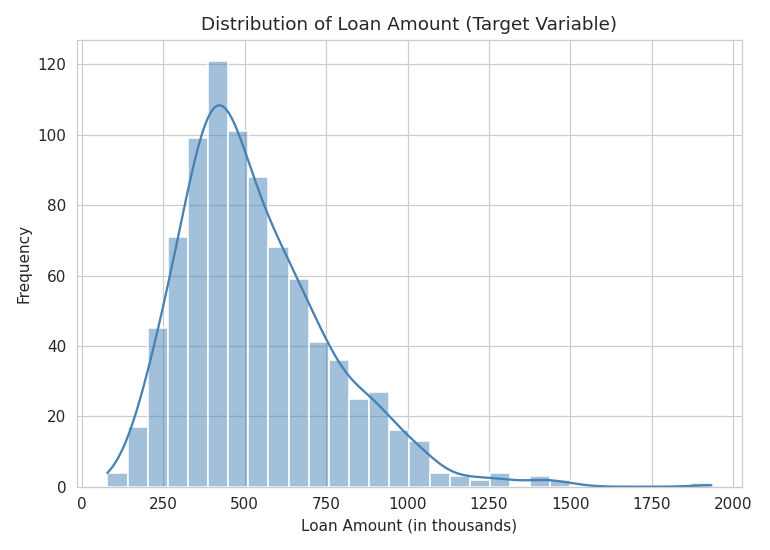
\includegraphics[width=0.65\linewidth]{01_target_distribution.png}
\caption{Distribution of the target variable, LoanAmount}
\end{figure}

\textbf{Inference:}

The loan amount distribution is right-skewed, with most sanctioned loans concentrated between
300 and 700 (in thousands) and a long tail of higher-value loans. Mean loan amount is
approximately 535 with a standard deviation of about 231. This skew is a signal to check the
residual plots later for heteroscedasticity, and it also motivates regularization, since a small
number of high-value samples can otherwise dominate coefficient estimates.

\subsection*{Feature vs. Target Scatter Plots}
\begin{figure}[H]
\centering
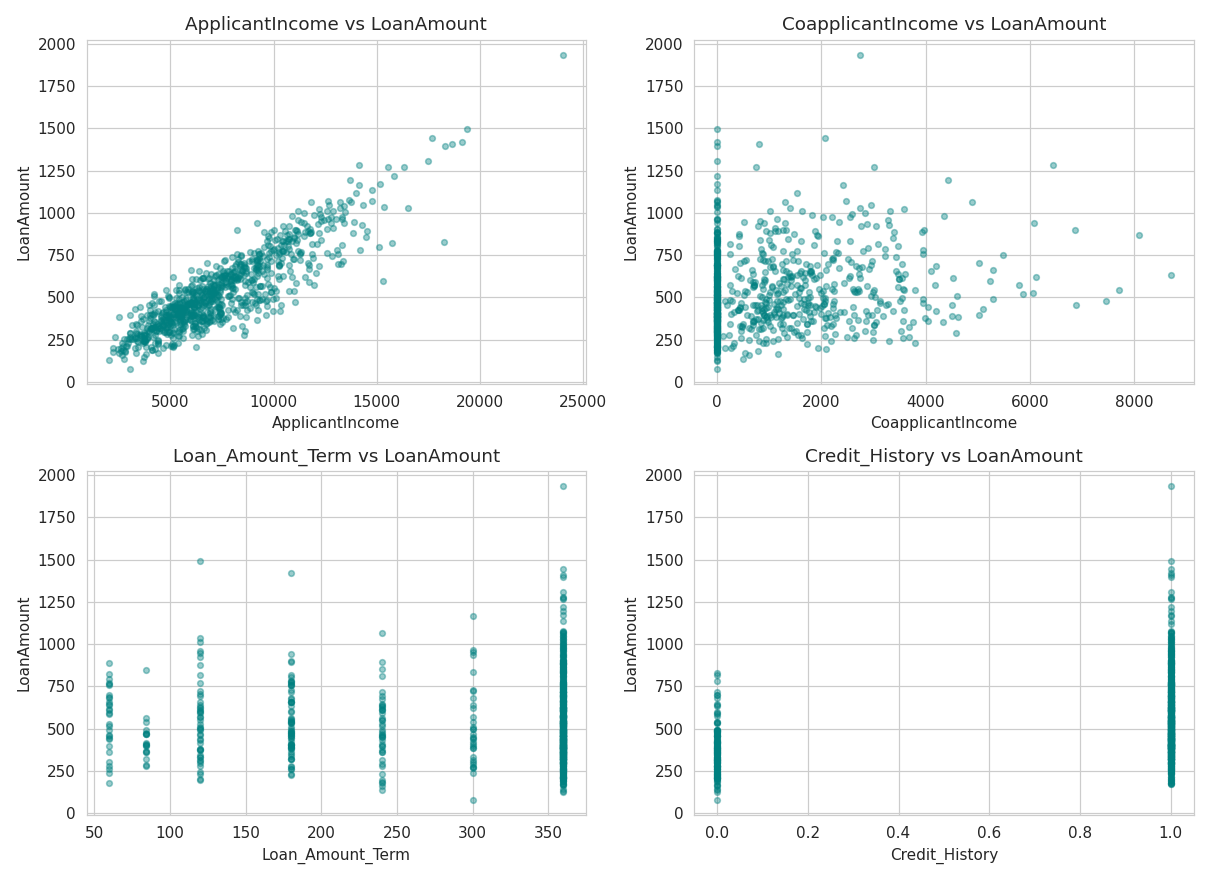
\includegraphics[width=0.85\linewidth]{02_feature_vs_target_scatter.png}
\caption{Numerical features plotted against LoanAmount}
\end{figure}

\textbf{Inference:}

\texttt{ApplicantIncome} shows the clearest positive linear relationship with \texttt{LoanAmount},
consistent with loan sizing being driven primarily by applicant income. \texttt{CoapplicantIncome}
shows a weaker but still positive trend. \texttt{Loan\_Amount\_Term} and \texttt{Credit\_History}
are close to discrete-valued and show little direct linear association with the target when
viewed alone, though \texttt{Credit\_History} interacts with other features in the fitted models.

\subsection*{Correlation Matrix}
\begin{figure}[H]
\centering
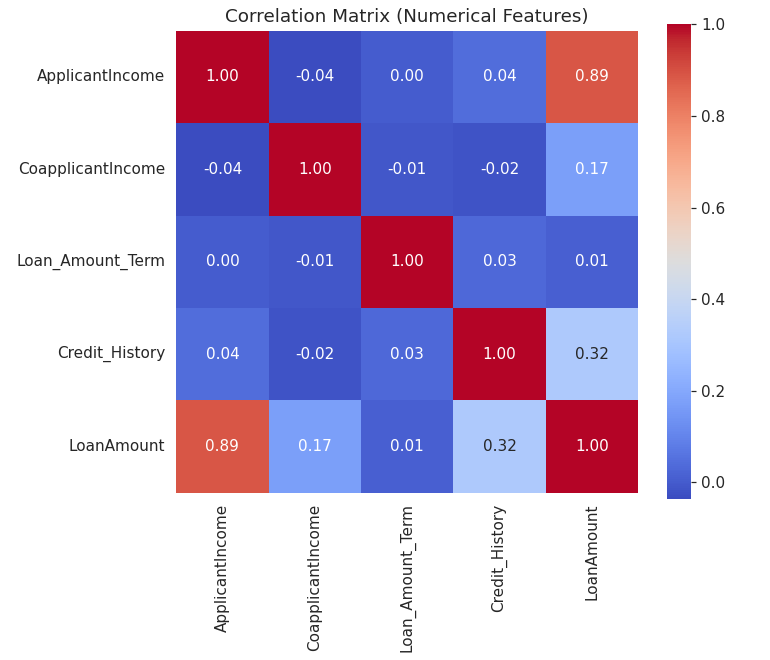
\includegraphics[width=0.55\linewidth]{03_correlation_matrix.png}
\caption{Correlation matrix of numerical features and the target}
\end{figure}

\textbf{Inference:}

\texttt{ApplicantIncome} correlates most strongly with \texttt{LoanAmount}, while
\texttt{CoapplicantIncome} contributes a smaller positive correlation. \texttt{Loan\_Amount\_Term}
and \texttt{Credit\_History} are weakly correlated with the target and with each other, indicating
limited multicollinearity among the numerical predictors -- a favorable condition for both
unregularized and regularized linear models.

\subsection*{Categorical Feature Distributions}
\begin{figure}[H]
\centering
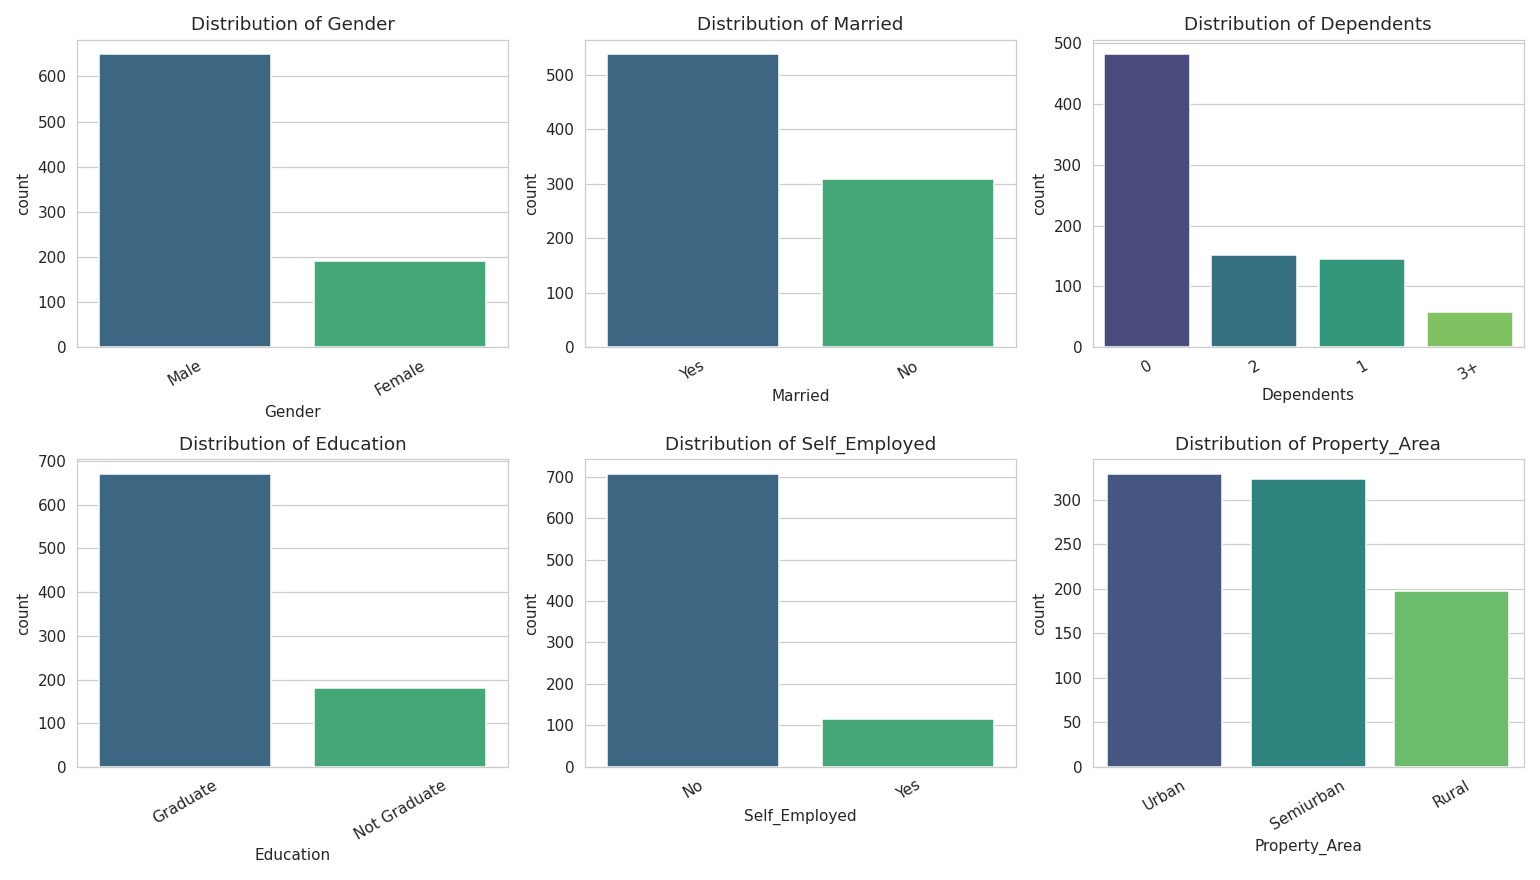
\includegraphics[width=0.9\linewidth]{04_categorical_distributions.png}
\caption{Distribution of categorical applicant features}
\end{figure}

\textbf{Inference:}

The applicant pool is predominantly male, married, graduate, and not self-employed, with most
applicants reporting no dependents and fairly balanced representation across the three property
area categories. This imbalance is handled through one-hot encoding but should be kept in mind when
interpreting the coefficients of minority categories, which are estimated from fewer supporting
samples.

\section{Data Preprocessing}

\begin{itemize}
\item \textbf{Missing value handling:} Numerical features (\texttt{ApplicantIncome},
\texttt{CoapplicantIncome}, \texttt{Loan\_Amount\_Term}, \texttt{Credit\_History}) were imputed
using the \textbf{median} of each column; categorical features (\texttt{Gender}, \texttt{Married},
\texttt{Dependents}, \texttt{Education}, \texttt{Self\_Employed}, \texttt{Property\_Area}) were
imputed using the \textbf{most frequent} category, both applied within a
\texttt{scikit-learn} \texttt{ColumnTransformer} pipeline fitted only on the training split to
avoid data leakage.
\item \textbf{Encoding:} Categorical features were transformed with \texttt{OneHotEncoder}
(\texttt{drop='first'}, \texttt{handle\_unknown='ignore'}), producing 10 encoded categorical
columns in addition to the 4 numerical columns (14 total model inputs).
\item \textbf{Feature scaling:} Numerical features were standardized with \texttt{StandardScaler}
(zero mean, unit variance) fitted on the training set only.
\item \textbf{Train-test split:} An 80/20 train-test split was used (\texttt{random\_state=42}),
giving 680 training samples and 170 test samples.
\item \textbf{Feature engineering:} No additional engineered features were created; the raw
applicant and loan attributes were used directly after imputation, encoding, and scaling.
\end{itemize}

\section{Machine Learning Algorithm}

\subsection*{Linear Regression}
\textbf{Working principle:} Fits a linear function of the input features that minimizes the sum of
squared residuals between predicted and actual values.

\textbf{Mathematical formulation:}
\[
\hat{y} = \beta_0 + \sum_{i=1}^{p}\beta_i x_i, \qquad
\hat{\beta} = \arg\min_{\beta}\sum_{j=1}^{n}\left(y_j - \beta_0 - \sum_{i=1}^{p}\beta_i x_{ji}\right)^2
\]

\textbf{Advantages:} Simple, interpretable, computationally cheap, serves as a strong baseline.

\textbf{Limitations:} No mechanism to control coefficient magnitude, so it can overfit or become
unstable when features are correlated or numerous relative to sample size.

\subsection*{Ridge Regression (L2 Regularization)}
\textbf{Working principle:} Adds a penalty proportional to the squared magnitude of the
coefficients, shrinking them toward zero without eliminating any.

\textbf{Mathematical formulation:}
\[
\hat{\beta}_{\text{ridge}} = \arg\min_{\beta}\left[\sum_{j=1}^{n}\left(y_j - \beta_0 -
\sum_{i=1}^{p}\beta_i x_{ji}\right)^2 + \alpha\sum_{i=1}^{p}\beta_i^2\right]
\]

\textbf{Advantages:} Reduces variance and stabilizes coefficient estimates under multicollinearity.

\textbf{Limitations:} Retains all features (no sparsity); requires tuning $\alpha$.

\subsection*{Lasso Regression (L1 Regularization)}
\textbf{Working principle:} Adds a penalty proportional to the absolute magnitude of the
coefficients, which can shrink some coefficients exactly to zero, performing implicit feature
selection.

\textbf{Mathematical formulation:}
\[
\hat{\beta}_{\text{lasso}} = \arg\min_{\beta}\left[\sum_{j=1}^{n}\left(y_j - \beta_0 -
\sum_{i=1}^{p}\beta_i x_{ji}\right)^2 + \alpha\sum_{i=1}^{p}|\beta_i|\right]
\]

\textbf{Advantages:} Produces sparse, more interpretable models by eliminating weak predictors.

\textbf{Limitations:} Can be unstable when features are highly correlated (tends to arbitrarily
pick one of a correlated group); requires tuning $\alpha$.

\subsection*{Elastic Net Regression}
\textbf{Working principle:} Combines the L1 and L2 penalties, blending Ridge's stability with
Lasso's sparsity via a mixing parameter.

\textbf{Mathematical formulation:}
\[
\hat{\beta}_{\text{enet}} = \arg\min_{\beta}\left[\sum_{j=1}^{n}\left(y_j - \beta_0 -
\sum_{i=1}^{p}\beta_i x_{ji}\right)^2 + \alpha\left(l1\_ratio\sum_{i=1}^{p}|\beta_i| +
\frac{1-l1\_ratio}{2}\sum_{i=1}^{p}\beta_i^2\right)\right]
\]

\textbf{Advantages:} More flexible than pure Ridge or Lasso; handles correlated features better
than Lasso alone while still allowing some sparsity.

\textbf{Limitations:} Two hyperparameters ($\alpha$, $l1\_ratio$) to tune, increasing search cost.

\section{Experimental Setup}
\begin{tabular}{ll}
\toprule
Python Version & 3.12.3 \\
Scikit-Learn Version & 1.8.0 \\
IDE & Jupyter Notebook \\
Operating System & Linux (Ubuntu 24.04) \\
Hardware & Standard CPU-based execution environment \\
\bottomrule
\end{tabular}

\section{Hyperparameter Selection}

\begin{tabular}{ll}
\toprule
Parameter & Value\\
\midrule
Ridge: $\alpha$ search space & \{0.01, 0.1, 1, 10, 100\} \\
Lasso: $\alpha$ search space & \{0.001, 0.01, 0.1, 1, 10\} \\
Elastic Net: $\alpha$ search space & \{0.01, 0.1, 1, 10\} \\
Elastic Net: $l1\_ratio$ search space & \{0.2, 0.5, 0.8\} \\
Cross-validation & 5-Fold (\texttt{KFold}, shuffle=True, random\_state=42) \\
Search method & \texttt{GridSearchCV} (scoring = R2) \\
\bottomrule
\end{tabular}

\subsection*{Hyperparameter Tuning Results}
\begin{table}[H]
\centering
\caption{Hyperparameter Tuning Summary}
\begin{tabular}{llll}
\toprule
Model & Search Method & Best Parameters & Best CV R2 \\
\midrule
Ridge Regression & Grid Search & $\alpha = 1$ & 0.9688 \\
Lasso Regression & Grid Search & $\alpha = 0.1$ & 0.9689 \\
Elastic Net Regression & Grid Search & $\alpha = 0.01$, $l1\_ratio = 0.8$ & 0.9688 \\
\bottomrule
\end{tabular}
\end{table}

\section{Results}

\subsection*{Cross-Validation Performance (K = 5, Training Set)}
\begin{table}[H]
\centering
\caption{Cross-Validation Performance}
\begin{tabular}{lcccc}
\toprule
Model & MAE & MSE & RMSE & R2 \\
\midrule
Linear Regression & 27.764 & 1500.399 & 38.735 & 0.9688 \\
Ridge Regression & 27.795 & 1500.700 & 38.739 & 0.9688 \\
Lasso Regression & 27.722 & 1498.476 & 38.710 & 0.9689 \\
Elastic Net Regression & 27.794 & 1500.670 & 38.738 & 0.9688 \\
\bottomrule
\end{tabular}
\end{table}

\subsection*{Test Set Performance}
\begin{table}[H]
\centering
\caption{Test Set Performance}
\begin{tabular}{lcccc}
\toprule
Model & MAE & MSE & RMSE & R2 \\
\midrule
Linear Regression & 31.623 & 1855.729 & 43.078 & 0.9705 \\
Ridge Regression & 31.588 & 1849.017 & 43.000 & 0.9706 \\
Lasso Regression & 31.540 & 1848.046 & 42.989 & 0.9706 \\
Elastic Net Regression & 31.573 & 1846.285 & 42.968 & 0.9706 \\
\bottomrule
\end{tabular}
\end{table}

\begin{table}[H]
\centering
\caption{Summary Metrics (Test Set) Including Training Time}
\begin{tabular}{lc}
\toprule
Metric & Best Model (Elastic Net Regression) \\
\midrule
MAE & 31.573 \\
MSE & 1846.285 \\
RMSE & 42.968 \\
R2 Score & 0.9706 \\
Training Time (s) & $\approx$ 0.4--1.0 \\
\bottomrule
\end{tabular}
\end{table}

\section{Result Visualization}

Include all graphs generated during the experiment.

\begin{figure}[H]
\centering
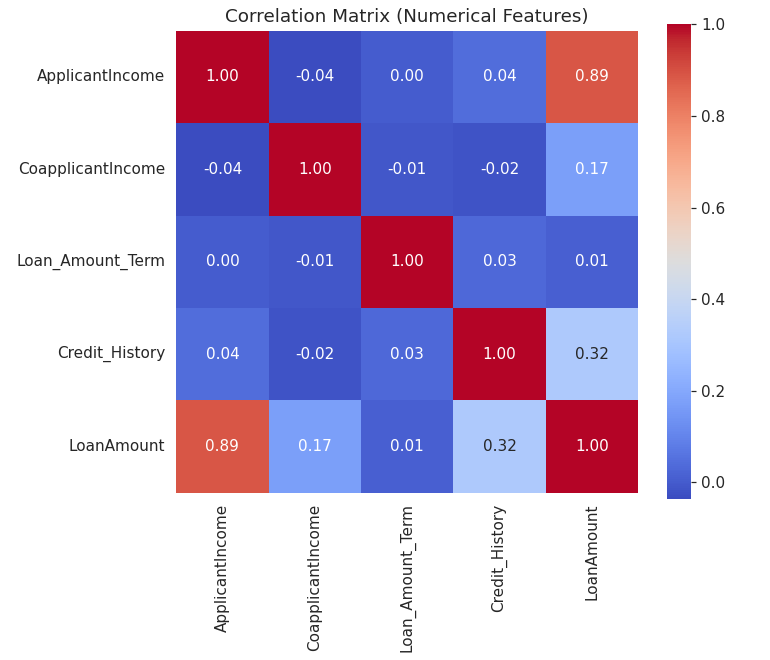
\includegraphics[width=0.55\linewidth]{03_correlation_matrix.png}
\caption{Correlation Matrix of numerical features and target}
\end{figure}

\textbf{Inference:} As discussed in the EDA section, \texttt{ApplicantIncome} is the dominant
numerically correlated predictor of \texttt{LoanAmount}, while inter-feature correlations remain
low, indicating minimal multicollinearity among numeric inputs.

\begin{figure}[H]
\centering
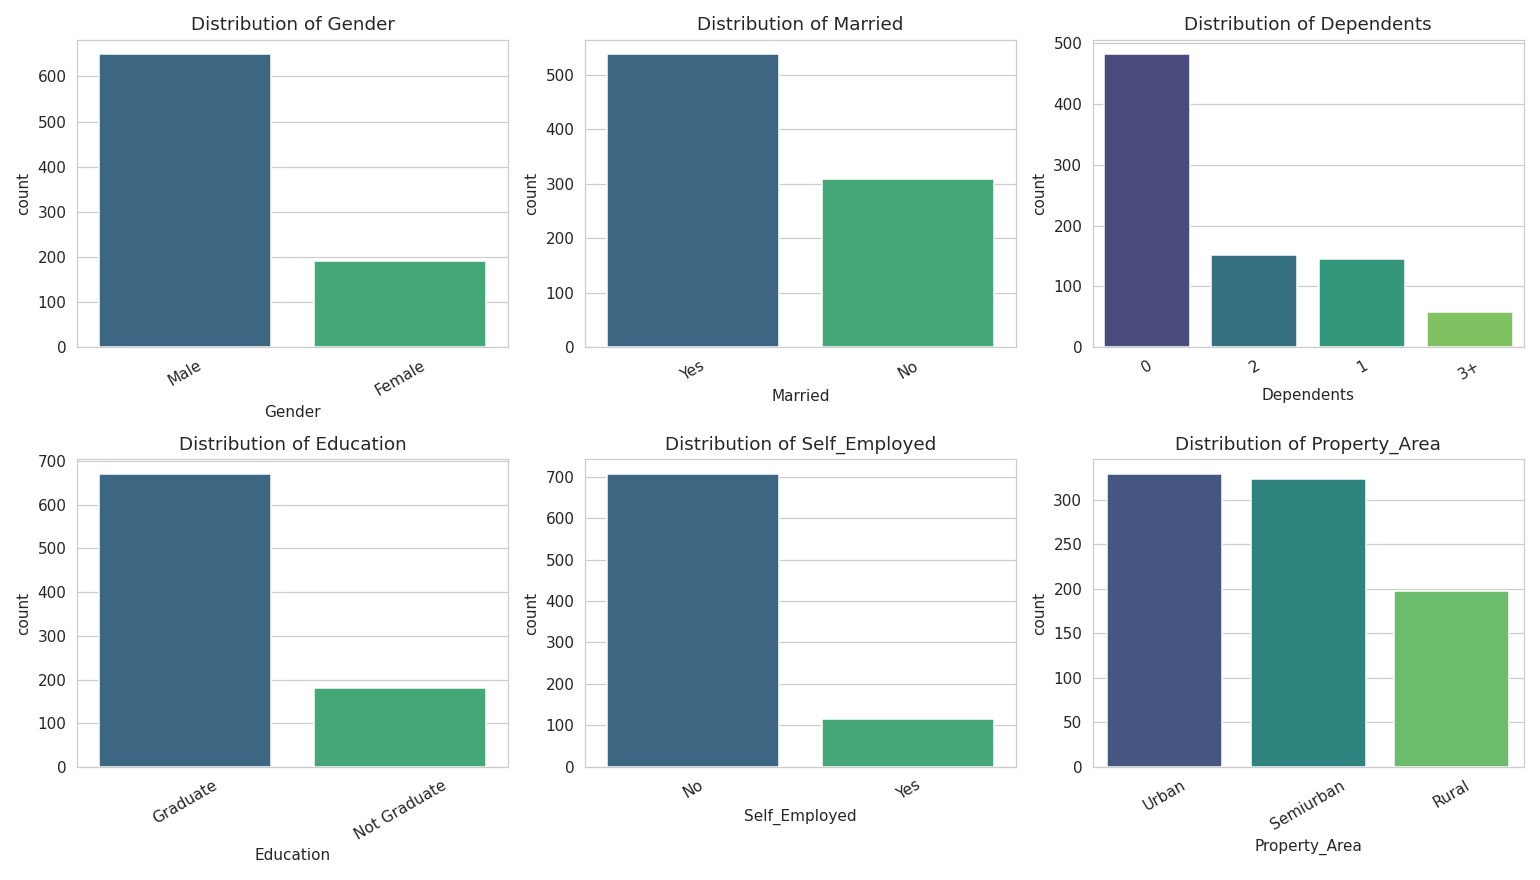
\includegraphics[width=0.9\linewidth]{04_categorical_distributions.png}
\caption{Class distribution of categorical applicant attributes}
\end{figure}

\textbf{Inference:} Category imbalance (e.g., far more married, graduate applicants with no
dependents) is visible across several categorical features; one-hot encoding with a dropped
reference level was used to accommodate this without introducing multicollinearity from the
dummy-variable trap.

\begin{figure}[H]
\centering
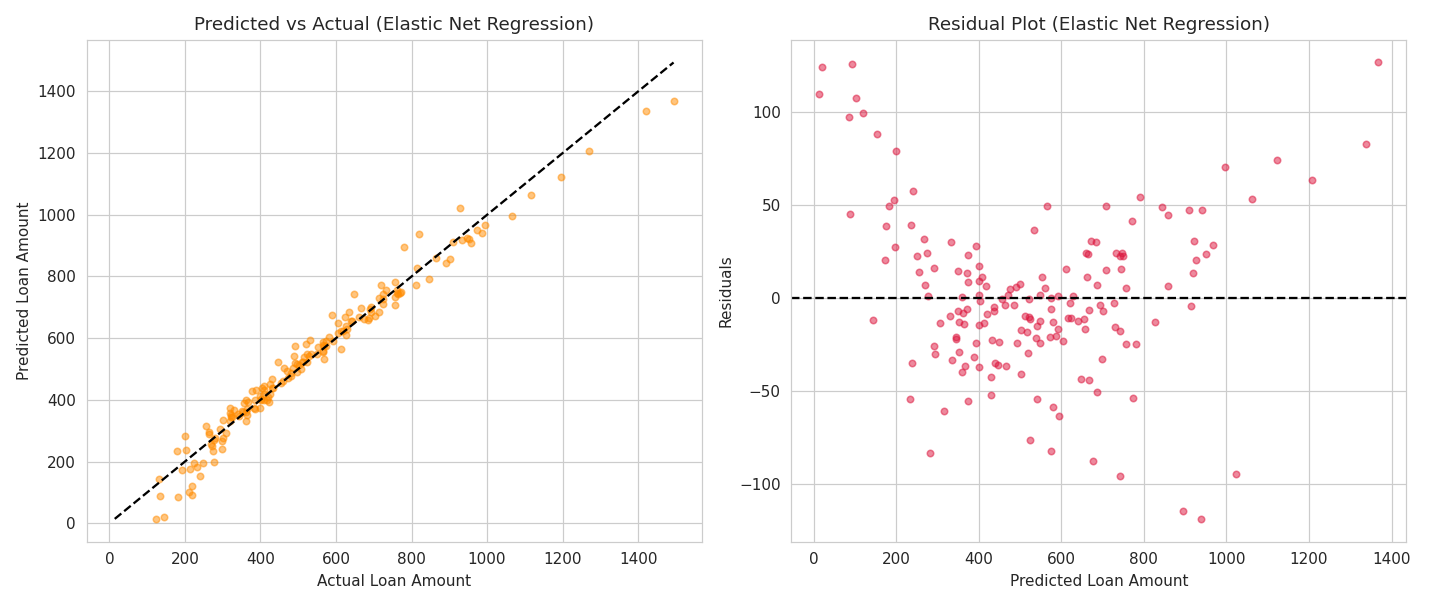
\includegraphics[width=0.95\linewidth]{05_predicted_vs_actual_residual.png}
\caption{Predicted vs. Actual values and Residual plot for the best model (Elastic Net Regression)}
\end{figure}

\textbf{Inference:} Predicted values track the actual loan amounts closely along the diagonal
reference line, confirming a strong fit (test $R^2 \approx 0.971$). Residuals are scattered
randomly around zero with no strong funnel shape, suggesting roughly constant error variance,
though a few larger residuals appear at higher predicted values, consistent with the right-skewed
target distribution.

\begin{figure}[H]
\centering
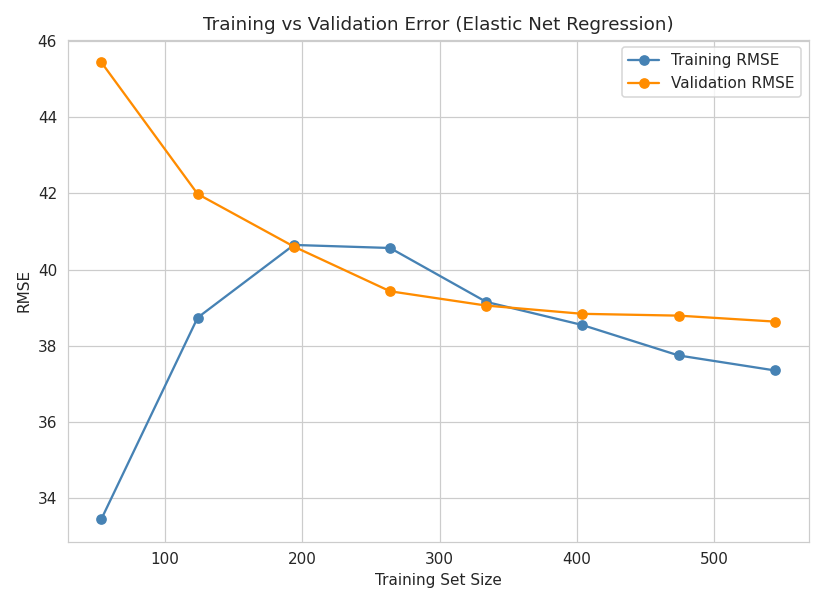
\includegraphics[width=0.65\linewidth]{06_train_val_error_curve.png}
\caption{Training vs. Validation error (learning curve) for the best model}
\end{figure}

\textbf{Inference:} Training and validation RMSE converge closely as the training set size
increases, with only a small, stable gap remaining. This indicates the model is not significantly
overfitting and that additional training data would yield diminishing returns given the current
feature set.

\begin{figure}[H]
\centering
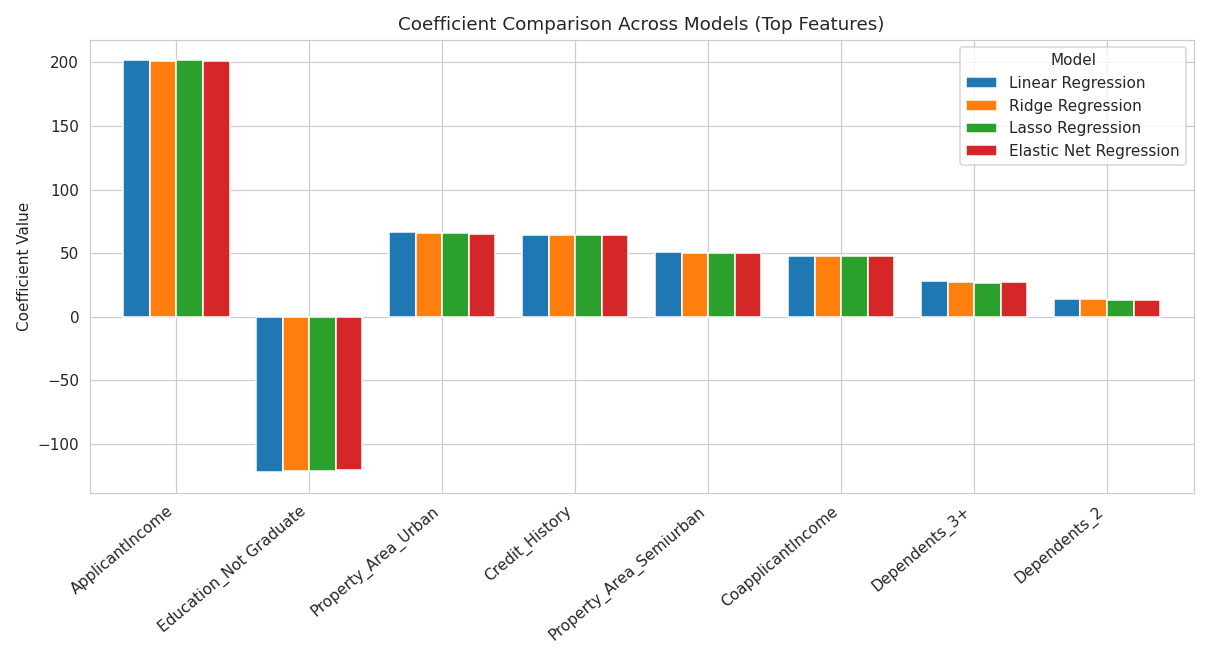
\includegraphics[width=0.9\linewidth]{07_coefficient_comparison.png}
\caption{Coefficient comparison across Linear, Ridge, Lasso, and Elastic Net (top features)}
\end{figure}

\textbf{Inference:} \texttt{ApplicantIncome} has by far the largest positive coefficient across all
four models ($\approx$ 201), confirming it as the dominant driver of loan amount. Ridge shrinks
coefficients only slightly relative to plain Linear Regression, while Lasso and Elastic Net shrink
smaller coefficients (e.g. \texttt{Dependents\_2}, \texttt{Dependents\_3+}) further toward zero,
illustrating Lasso's feature-sparsity behavior.

\begin{table}[H]
\centering
\caption{Coefficient Comparison (Top Features)}
\begin{tabular}{lcccc}
\toprule
Feature & Linear & Ridge & Lasso & Elastic Net \\
\midrule
ApplicantIncome & 201.60 & 201.30 & 201.50 & 201.18 \\
Education\_Not Graduate & -122.16 & -121.13 & -121.66 & -120.72 \\
Property\_Area\_Urban & 66.61 & 65.69 & 65.56 & 65.29 \\
Credit\_History & 64.15 & 64.08 & 64.10 & 64.05 \\
Property\_Area\_Semiurban & 51.22 & 50.40 & 50.17 & 50.02 \\
CoapplicantIncome & 47.73 & 47.59 & 47.72 & 47.54 \\
Dependents\_3+ & 28.08 & 27.55 & 26.26 & 27.23 \\
Dependents\_2 & 13.92 & 13.67 & 12.89 & 13.51 \\
\bottomrule
\end{tabular}
\end{table}

\begin{figure}[H]
\centering
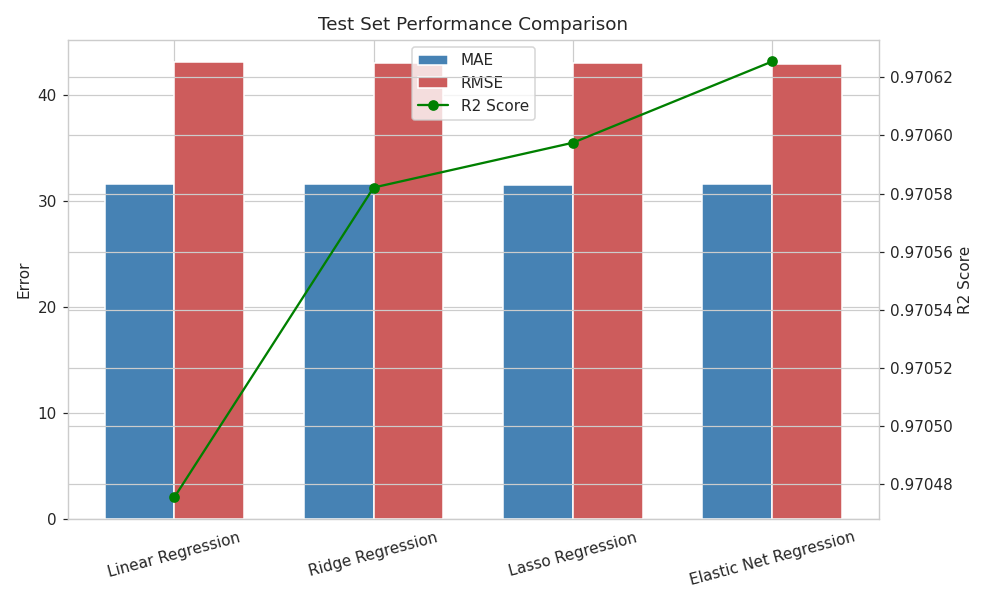
\includegraphics[width=0.75\linewidth]{08_test_performance_comparison.png}
\caption{Test set performance comparison (MAE, RMSE, R2) across all four models}
\end{figure}

\textbf{Inference:} All four models perform almost identically on the held-out test set
($R^2 \approx 0.9705$--$0.9706$), with Elastic Net marginally ahead on RMSE and R2. This suggests
the dataset's linear signal is strong and clean enough that regularization mainly stabilizes
coefficients rather than materially changing predictive accuracy.

\section{Discussion}

Across all four models, test-set $R^2$ is consistently around 0.970--0.971, and the gap between
5-fold cross-validated training performance and test performance is small (e.g. CV RMSE
$\approx$ 38.7 vs. test RMSE $\approx$ 43.0), indicating the models generalize well rather than
memorizing the training data. Grid search consistently selected small regularization strengths
(Ridge $\alpha=1$, Lasso $\alpha=0.1$, Elastic Net $\alpha=0.01$), which is expected given the low
multicollinearity observed in the correlation matrix -- there is limited redundant information for
regularization to compress. The main strength of this experiment is the clear, consistent
dominance of \texttt{ApplicantIncome} as a predictor across every model, which makes the results
easy to interpret. A limitation is that, because the numeric predictors are only weakly correlated
with each other, the practical benefit of Ridge/Lasso/Elastic Net over plain Linear Regression is
small on this particular dataset; the advantage of regularization would likely be more pronounced
on a noisier dataset with more correlated or higher-dimensional features. Potential improvements
include engineering an income-to-loan-term ratio feature, exploring polynomial or interaction
terms, and testing tree-based models (e.g. Random Forest, Gradient Boosting) as a non-linear
comparison baseline.

\section{Conclusion}

Linear Regression, Ridge, Lasso, and Elastic Net regression models were implemented and evaluated
for predicting sanctioned loan amount from applicant demographic and financial features. After
5-fold cross-validated grid search, all four models converged to very similar performance (test
$R^2 \approx 0.970$--$0.971$), with Elastic Net Regression ($\alpha=0.01$, $l1\_ratio=0.8$)
achieving the best test RMSE (42.968) and R2 (0.9706) by a narrow margin over Lasso and Ridge, and
all three regularized models slightly outperforming the unregularized baseline. The small,
converging training-validation error gap observed in the learning curve confirms the models are
neither substantially overfitting nor underfitting. Given the near-identical accuracy, Elastic Net
or Ridge would be the preferred choice in practice for their added coefficient stability, at
essentially no cost in predictive accuracy, over plain Linear Regression.

\section{References}
\begin{enumerate}
\item Scikit-learn Developers, ``Linear Models,'' \textit{scikit-learn documentation}.
\url{https://scikit-learn.org/stable/modules/linear_model.html}
\item Scikit-learn Developers, ``Tuning the hyper-parameters of an estimator,'' \textit{scikit-learn documentation}.
\url{https://scikit-learn.org/stable/modules/grid_search.html}
\item Kaggle, ``Predict Loan Amount Data'' dataset.
\end{enumerate}

\end{document}
